\documentclass[12pt]{article}
\usepackage[utf8]{inputenc}
\newenvironment{sol}[1][Solution]{\begin{trivlist}\item[\hskip\labelsep {\bfseries #1:}]}{\end{trivlist}}
\usepackage[margin=1in]{geometry} 
\usepackage{amsmath,amsthm,amssymb}
\usepackage{color}
\usepackage{minted}
\usepackage{graphicx}
\title{Southern Methodist University \\
Bobby B. Lyle School of Engineering Department of Computer Science \\
Homework 3
}
\usepackage{times,url}   
\author{Operating System and Software System \\
Name: Bingying Liang 
\\ ID: 48999397\\ 
Email: bingyingl@smu.edu \\ 
CS7343 Distance}
\date{Feb 28 2023}

\begin{document}
\maketitle
\begin{enumerate}
    \item This question involves implementing several different process scheduling algorithms. The scheduler will be assigned a predefined set of tasks and will schedule the tasks based on the selected scheduling algorithm. Each task is assigned a priority and CPU burst.\\
    The following scheduling algorithms will be implemented:
    \begin{enumerate}
        \item First-come, first-served (FCFS), which schedules tasks in the order in which they request the CPU.
        \item Shortest-job-first (SJF), which schedules tasks in order of the length of the tasks’ next CPU burst.
        \item Priority scheduling, which schedules tasks based on priority.
        \item Round-robin (RR) scheduling, where each task is run for a time quantum (or for the remainder of its CPU burst). 
        \item Priority with round-robin, which schedules tasks in order of priority and uses round-robin scheduling for tasks with equal priority.
    \end{enumerate}
    Note: Please see Page P-29 for a complete description of this Homework. There are supporting Java files for this assignment that will be provided in Canvas/Files/Homework3. You may choose any programming language that you would like for this homework, but it would be easier to implement in Java since the supporting files are all Java code. 
    
    P-29: Priorities range from 1 to 10, where a higher numeric value indicates a higher relative priority. For round-robin scheduling, the length of a time quantum is 10 milliseconds.\\
    \begin{sol}
    The implementation of this project completes in Java. Program supporting files are download from the textbook website. These supporting files read in the schedule of tasks, insert the tasks into a list, and invoke the scheduler.\\
    The schedule of tasks has the form $[\textbf{task name}][\textbf{priority}][\textbf{CPU burst}]$, with the following example format and store in file book.txt:
    \begin{align*}
        & T1, 4, 20 \\
        & T2, 2, 25 \\
        & T3, 3, 25 \\
        & T4, 3, 15 \\
        & T5, 10, 10 
    \end{align*}
    Thus, task T1 has priority 4 and a CPU burst of 20 milliseconds, and so forth. It is assume that all tasks arrive at the same time, so the scheduler algorithms do not have to support higher-priority processes preempting processes with lower priorities. In addition, task do not have to be placed into a queue or list in any particular order.
    The program is run as follows:
     \begin{minted}[frame=lines,framesep=2mm,baselinestretch=1.2,fontsize=\footnotesize]{shell}
     java Driver fcfs book.txt
    \end{minted}
    \begin{enumerate}
        \item First-come, first-served(FCFS)
             \begin{minted}[frame=lines,framesep=2mm,baselinestretch=1.2,fontsize=\footnotesize,linenos]{java}
import java.util.List;

public class FCFS implements Algorithm{
    private List<Task> queue;
    public FCFS(List<Task> queue){
        this.queue = queue;
    }

    @Override
    public void schedule() {
        System.out.println("First-come, first-served(FCFS): \n");
        while(queue.size() != 0){
            Task next = pickNetTask();
            queue.remove(next);
            CPU.run(next, next.getBurst());
            System.out.println("Task " + next.getName() 
                                + " finished.\n");
	    System.out.println("----------------------
                                -----------------");
        }
    }

    @Override
    public Task pickNetTask() {
        return queue.get(0);
    }
}
    \end{minted}
    Result:\\
     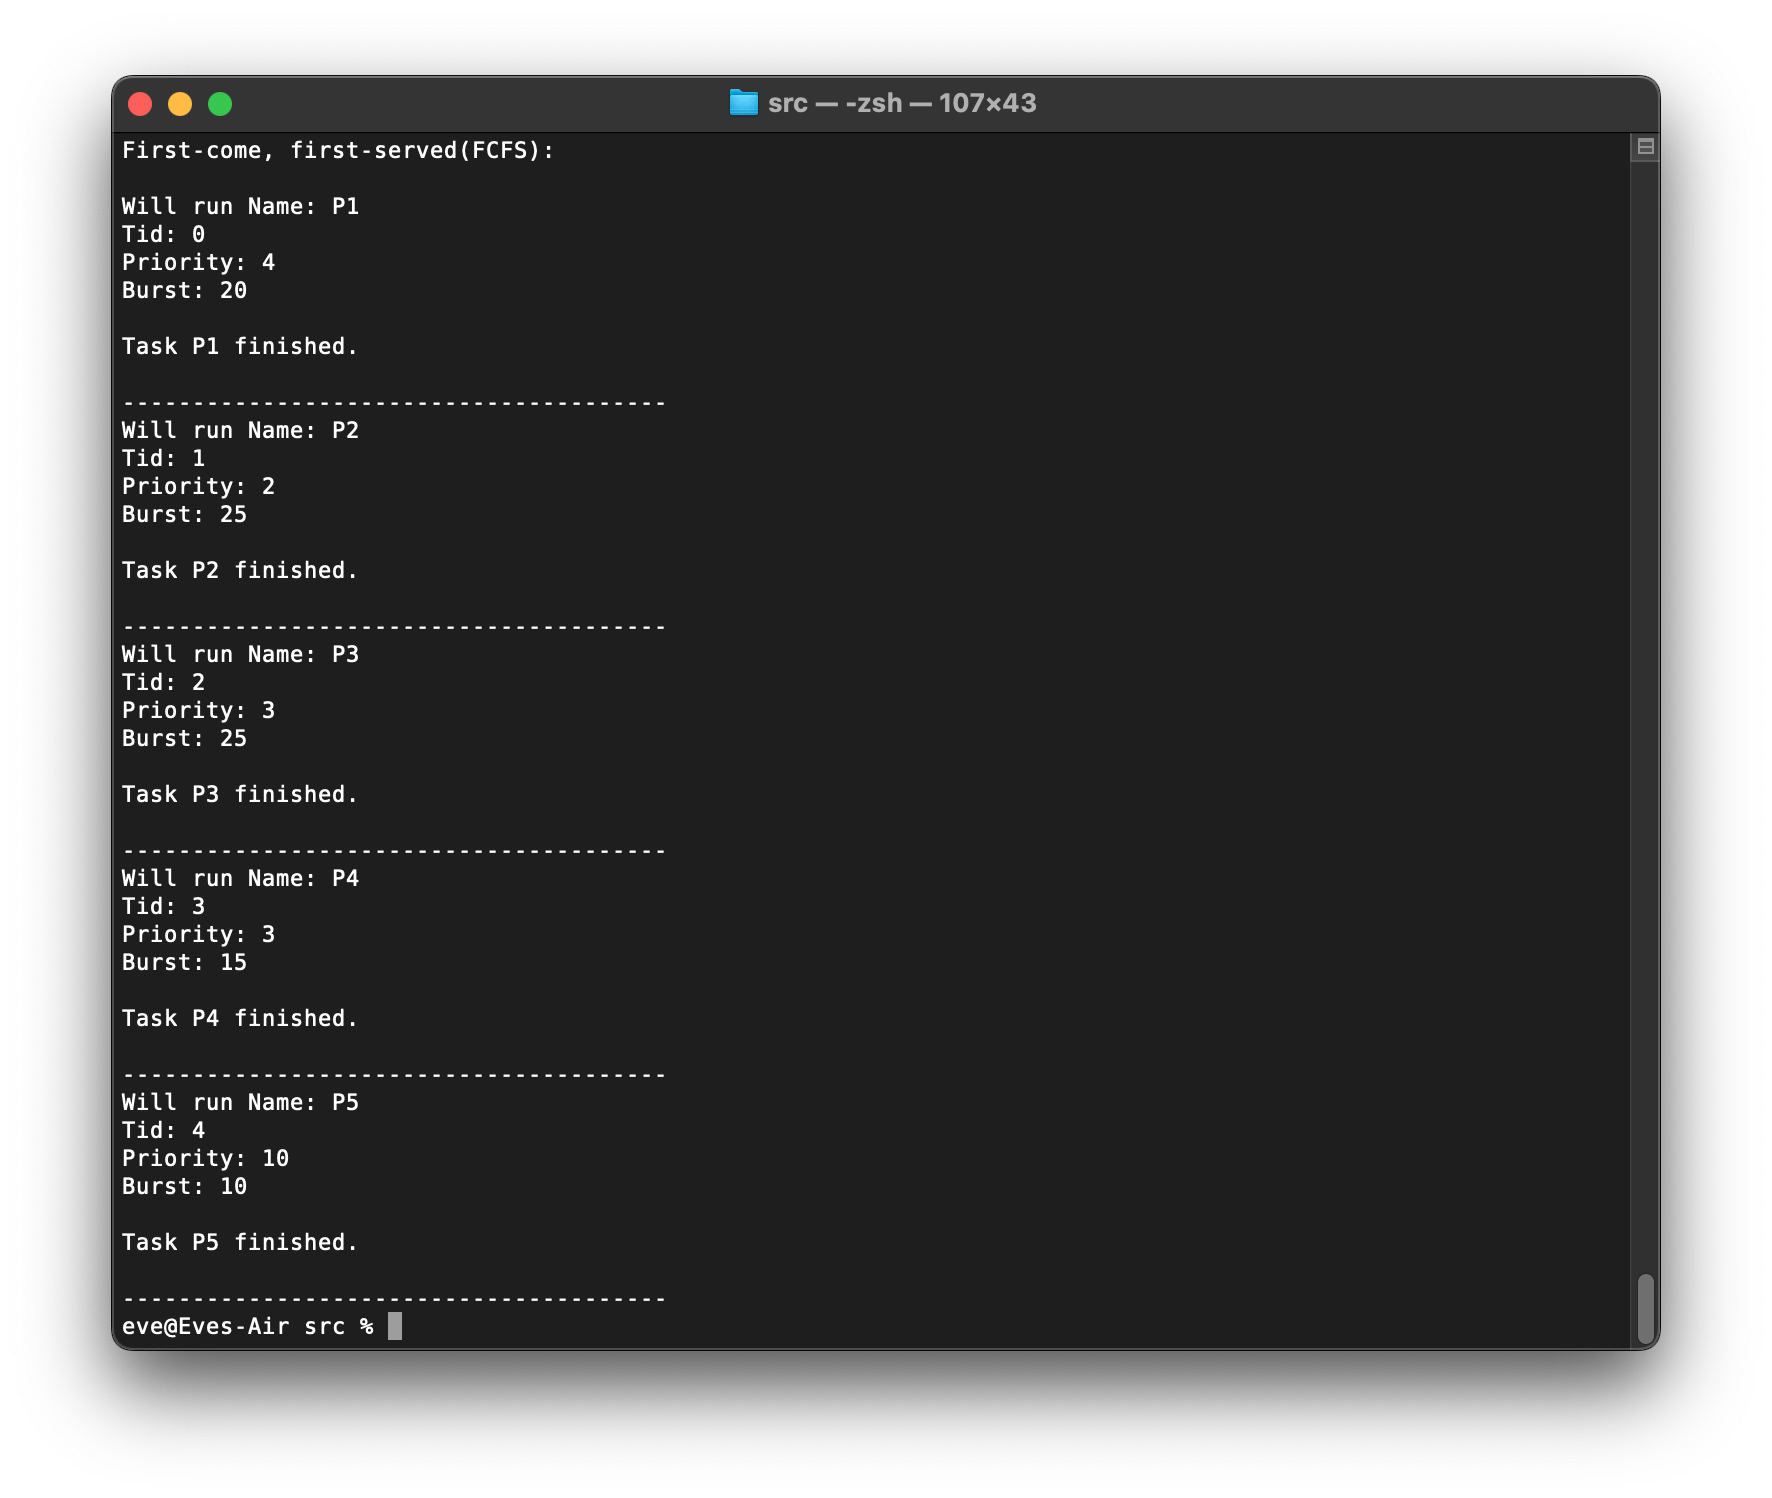
\includegraphics[width=0.9\textwidth]{a1.png}
    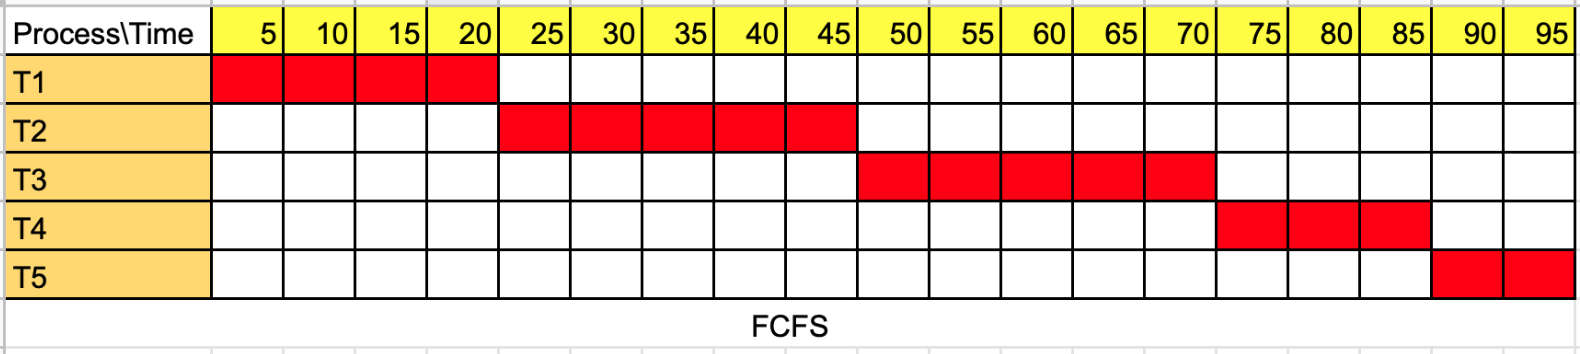
\includegraphics[width=0.9\textwidth]{P1.png}

    \item Shortest-job-first (SJF):
        \begin{minted}[frame=lines,framesep=2mm,baselinestretch=1.2,fontsize=\footnotesize,linenos]{java}
import java.util.List;

public class SJF implements Algorithm {
    private List<Task> queue;

    public SJF(List<Task> queue){
        this.queue = queue;
    }

    @Override
    public void schedule() {
        System.out.println("Shortest-job-first(SJF): \n");
        while(queue.size() != 0){
            Task next = pickNetTask();
            queue.remove(next);
            CPU.run(next, next.getBurst());
            System.out.println("Task " + next.getName() 
                                + " finished\n");
            System.out.println("-------------------
                                --------------------");
        }
    }

    @Override
    public Task pickNetTask() {
        // schedules tasks in order of 
        // the length of the tasks' next CPU burst.
        int Tid_index = -1;
        int min = Integer.MAX_VALUE;
        for (int i = 0; i < queue.size(); i++){
            int currentBurst = queue.get(i).getBurst();
            if (currentBurst < min){
                min = currentBurst;
                Tid_index = i;
            }
        }
        return queue.get(Tid_index);
    }
}
    \end{minted}
        Result:\\
    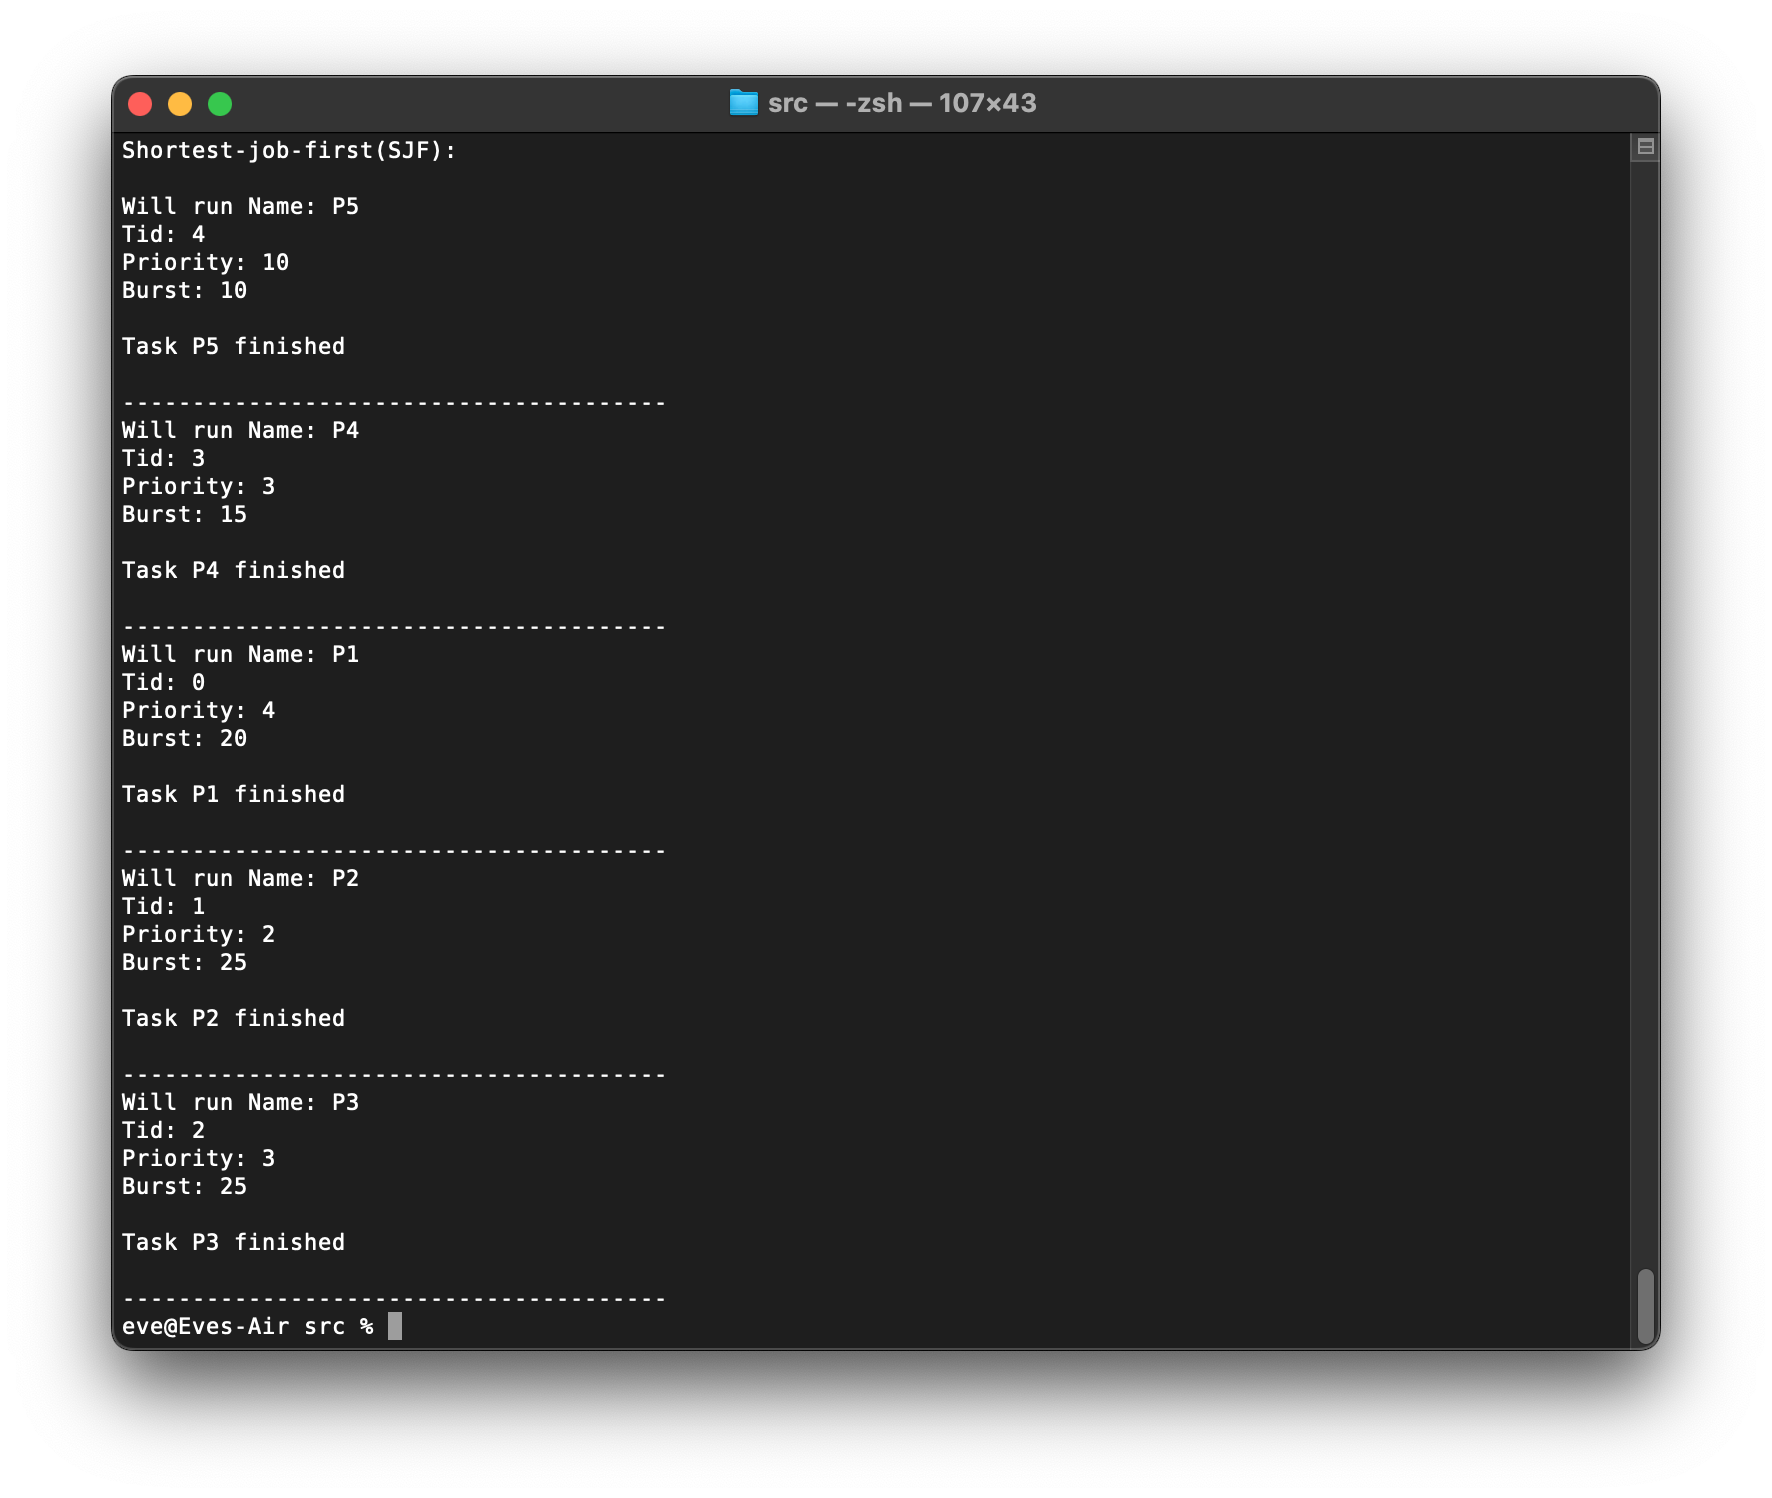
\includegraphics[width=0.9\textwidth]{a2.png}
    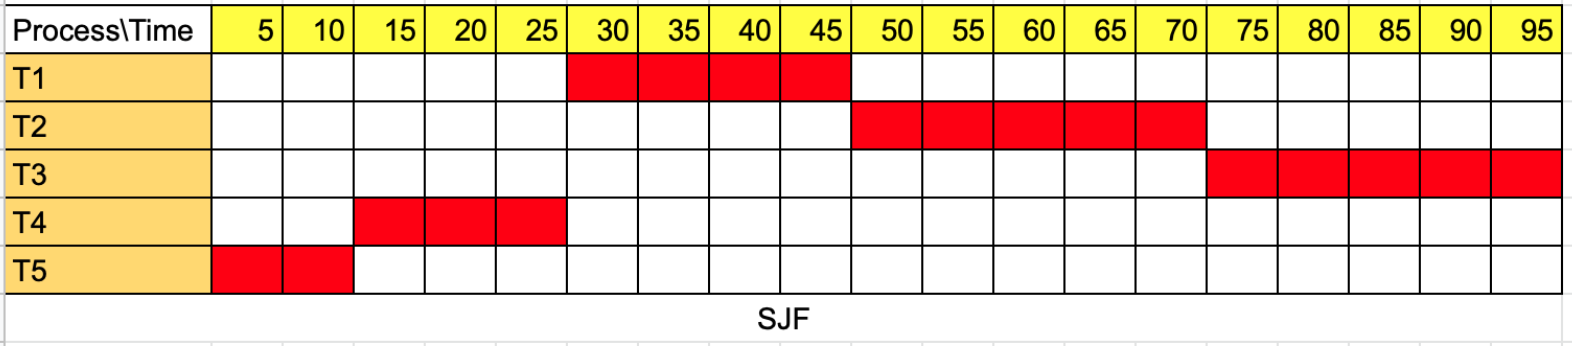
\includegraphics[width=0.9\textwidth]{P2.png}

    \item Priority scheduling:
        \begin{minted}[frame=lines,framesep=2mm,baselinestretch=1.2,fontsize=\footnotesize,linenos]{java}
import java.util.List;

public class Priority implements Algorithm {
    private List<Task> queue;

    public Priority(List<Task> queue){
        this.queue = queue;

    }

    @Override
    public void schedule() {
        System.out.println("Priority scheling:");
        while (queue.size() != 0){
            Task next = pickNetTask();
            queue.remove(next);
            CPU.run(next, next.getBurst());
            System.out.println("Task " + next.getName() 
                                + " finished\n");
            System.out.println("-----------------------
                                ----------------");
        }

    }

    @Override
    public Task pickNetTask() {
        // scheduling task based on priority
        // Priorities range from 1 to 10, where a higher numeric value 
        // indicates a higher relative priority.
        int Tid_index = -1;
        int max = Integer.MIN_VALUE;
        for (int i = 0; i < queue.size(); i++){
            int currentPriority = queue.get(i).getPriority();
            if (currentPriority > max){
                max = currentPriority;
                Tid_index = i;
            }
        }
        return queue.get(Tid_index);
    }
}
    \end{minted}
        Result:\\
    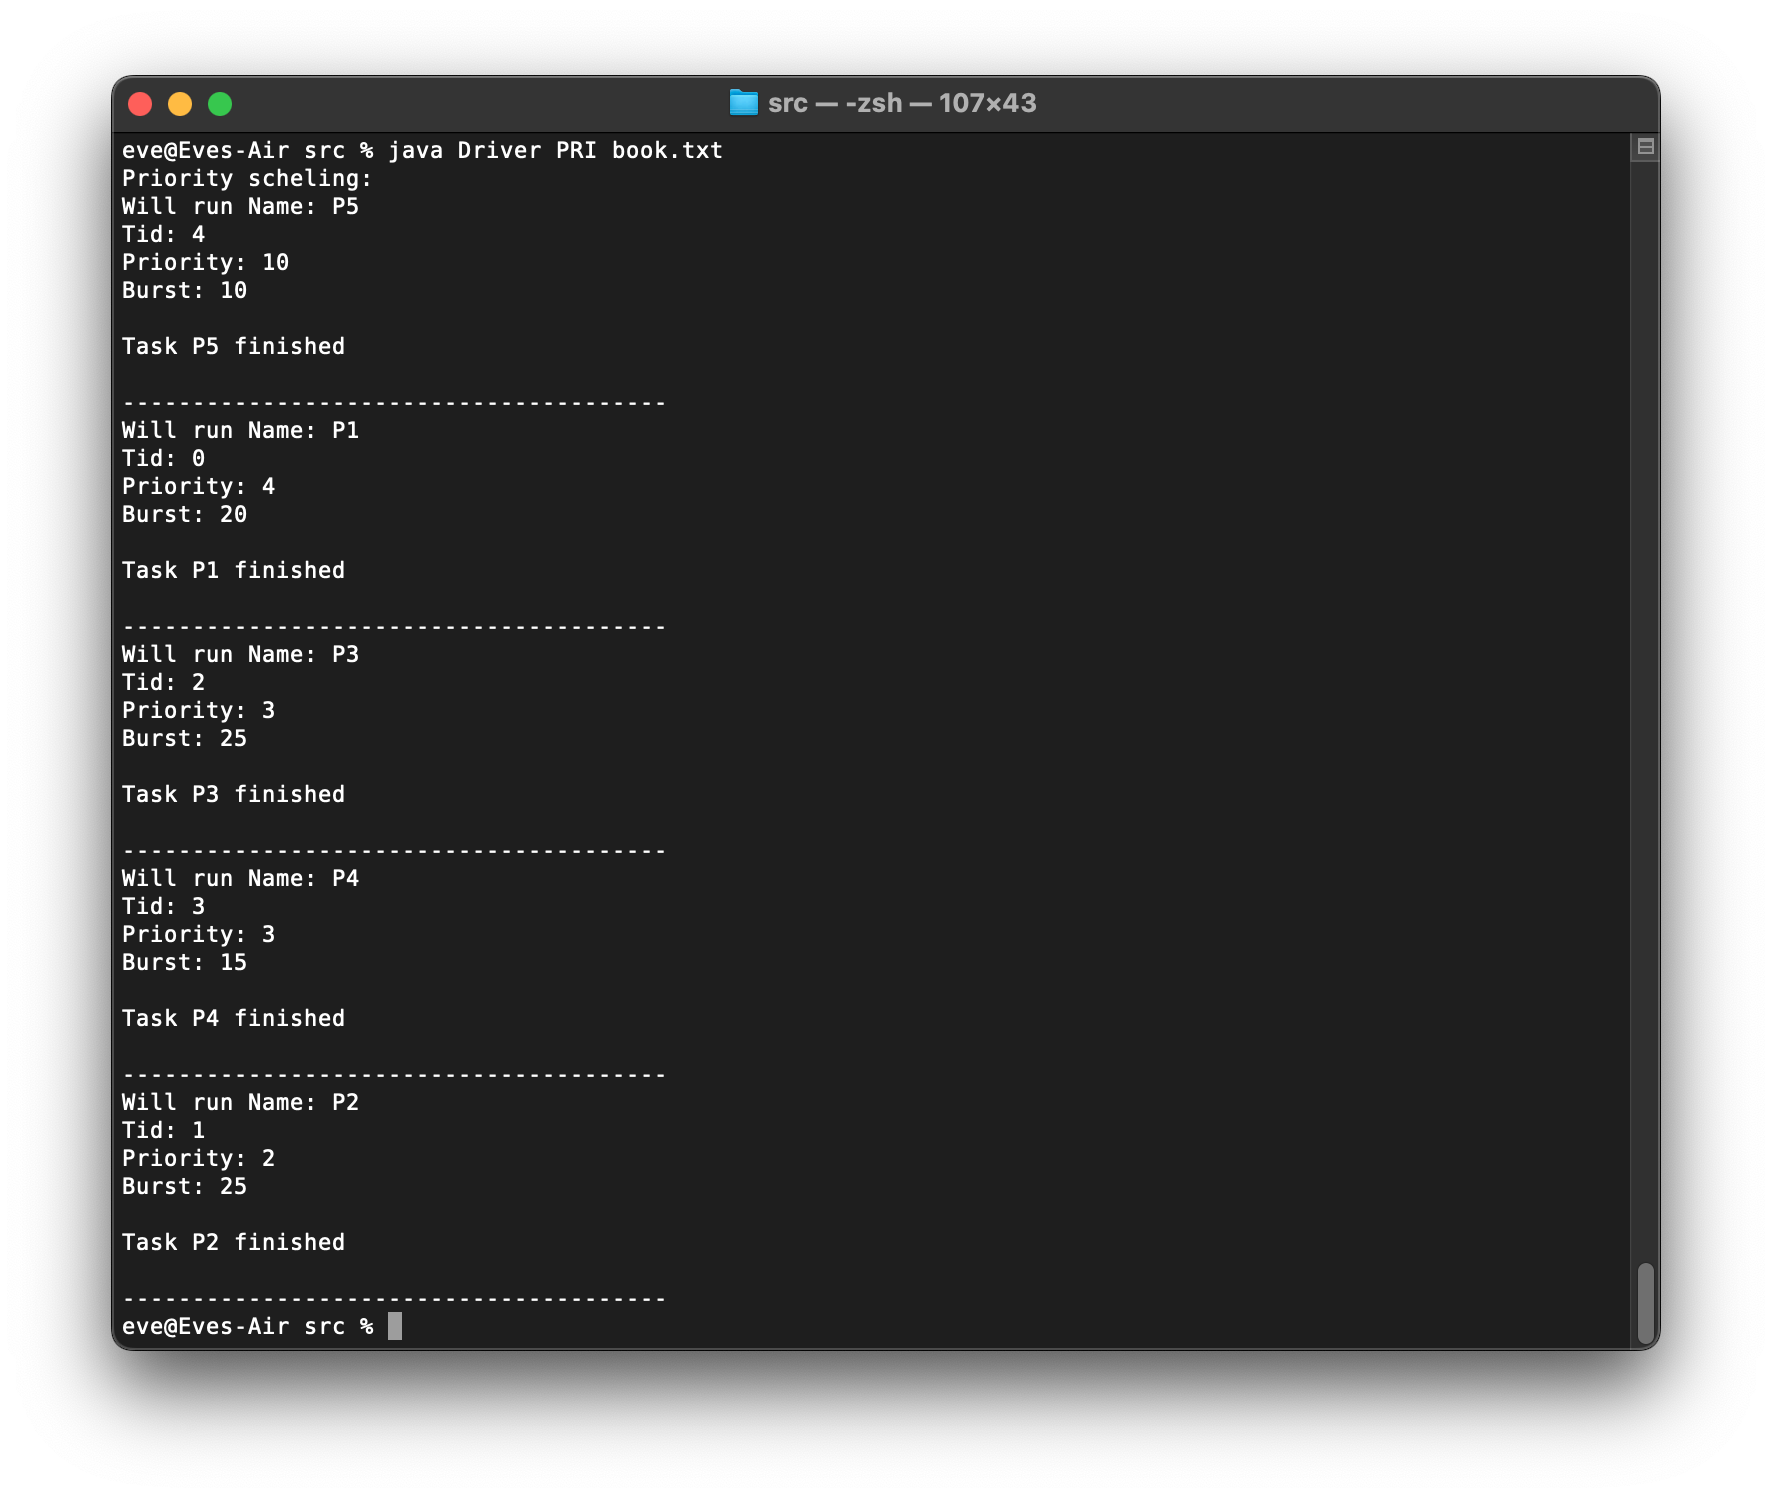
\includegraphics[width=0.9\textwidth]{a3.png}
    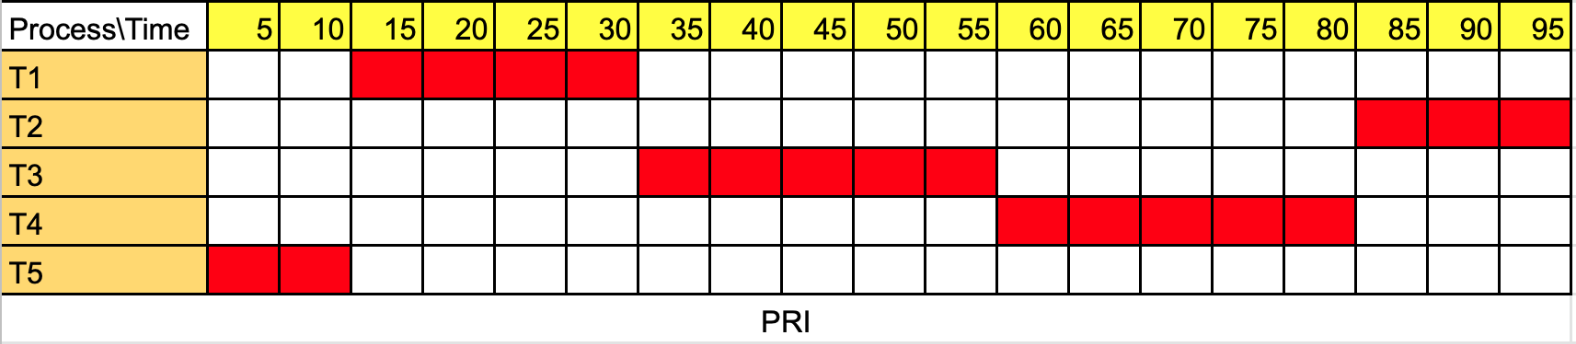
\includegraphics[width=0.9\textwidth]{P3.png}

    \item Round-robin (RR) Scheduling:
            \begin{minted}[frame=lines,framesep=2mm,baselinestretch=1.2,fontsize=\footnotesize,linenos]{java}
import java.util.List;

public class RR implements Algorithm{

    private List<Task> queue;
    int quantum = 10;

    public RR(List<Task> queue){
        this.queue = queue;
    }
    @Override
    public void schedule() {
        System.out.println("Round-robin (RR) scheduling: \n");
        while(queue.size() != 0){
            Task next = pickNetTask();
            queue.remove(next);
            if (next.getBurst() > quantum){
                CPU.run(next, quantum);
                next.setBurst(next.getBurst() - quantum);
                System.out.println(next.getName() + " has ran " 
                                    + quantum 
                                    + " and the remaining Burst is " 
                                    + next.getBurst() + "\n");
                queue.add(next);
                System.out.println("-----------------------------
                                -----------------------------------");
            } else {
                CPU.run(next, next.getBurst());
                System.out.println(next.getName() + " has ran " 
                                    + next.getBurst() 
                                    + " and the remaining Burst is 0\n");
                next.setBurst(0);
                System.out.println("Task " + next.getName() 
                                    + " finished\n");
                System.out.println("-------------------------
                        ----------------------------------------");
            }

        }
    }

    @Override
    public Task pickNetTask() {
        return queue.get(0);
    }
}

    \end{minted}
        Result:\\
    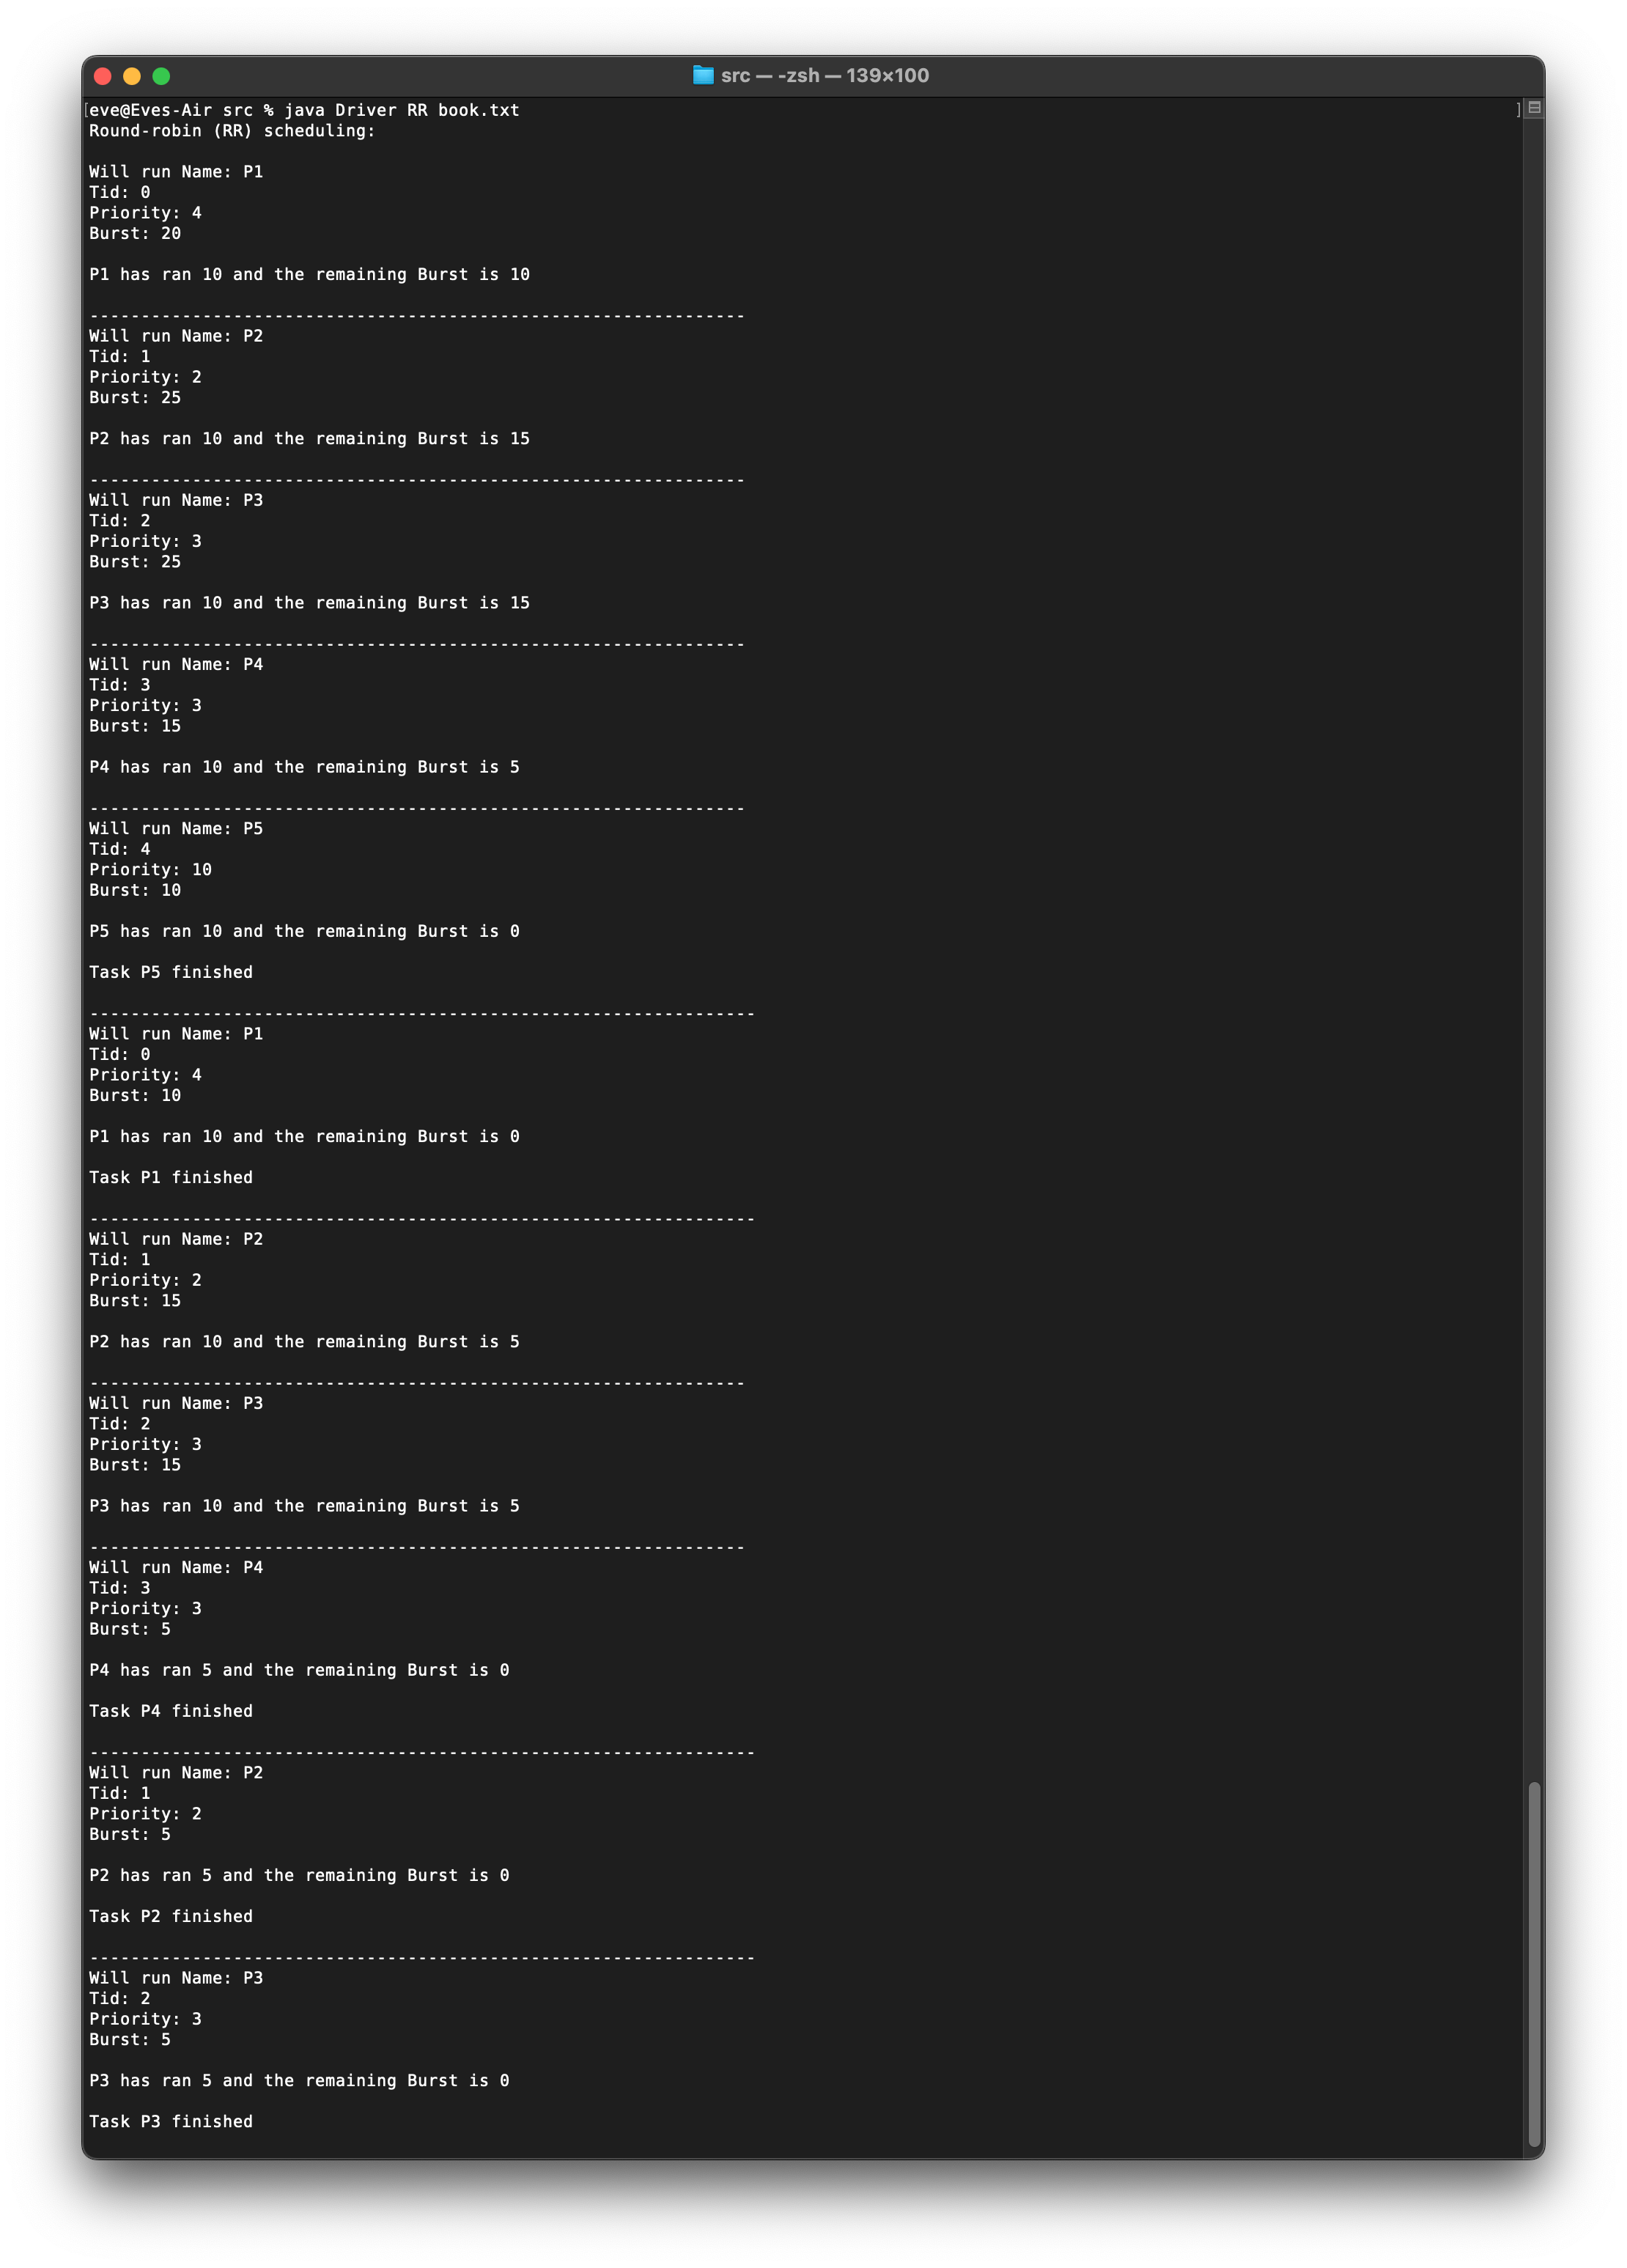
\includegraphics[width=0.9\textwidth]{a4.png}
    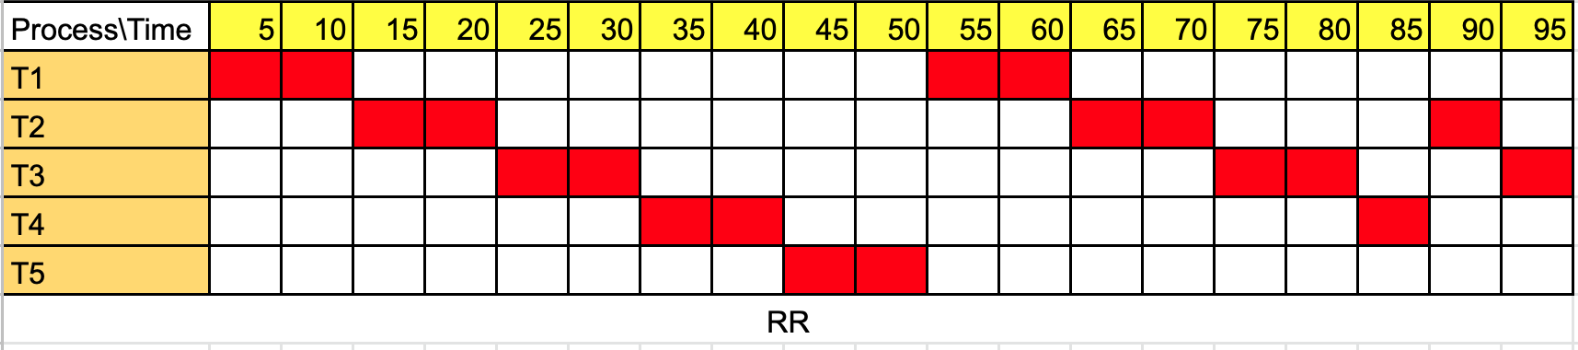
\includegraphics[width=0.9\textwidth]{P4.png}

    \item Priority with round-robin:
        \begin{minted}[frame=lines,framesep=2mm,baselinestretch=1.2,fontsize=\footnotesize,linenos]{java}
import java.util.List;

public class PriorityRR implements Algorithm{
    private List<Task> queue;
    int quantum = 10;

    public PriorityRR(List<Task> queue){
        this.queue = queue;
    }
    @Override
    public void schedule() {
        System.out.println("Priority with round-robin: \n");
        while(queue.size() != 0){
            Task next = pickNetTask();
            queue.remove(next);
            if (next.getBurst() > quantum){
                CPU.run(next, quantum);
                next.setBurst(next.getBurst() - quantum);
                System.out.println(next.getName() + " has ran " 
                                    + quantum 
                                    + " and the remaining Burst is " 
                                    + next.getBurst() + "\n");
                queue.add(next);
                System.out.println("--------------------------
                        --------------------------------------");
            } else {
                CPU.run(next, quantum);
                System.out.println(next.getName() + " has ran " 
                                + next.getBurst() 
                                + " and the remaining Burst is 0\n");
                next.setBurst(0);
                System.out.println("Task " + next.getName() 
                                    + " finished\n");
                System.out.println("-----------------------------
                            ------------------------------------");
            }
        }
    }
    
    @Override
    public Task pickNetTask() {
        int Tid_index = -1;
        int max = Integer.MIN_VALUE;
        for (int i = 0; i < queue.size(); i++){
            int currentPriority = queue.get(i).getPriority();
            if (currentPriority > max){
                max = currentPriority;
                Tid_index = i;
            }
        }
        return queue.get(Tid_index);
    }
}
    \end{minted}
        Result:\\
    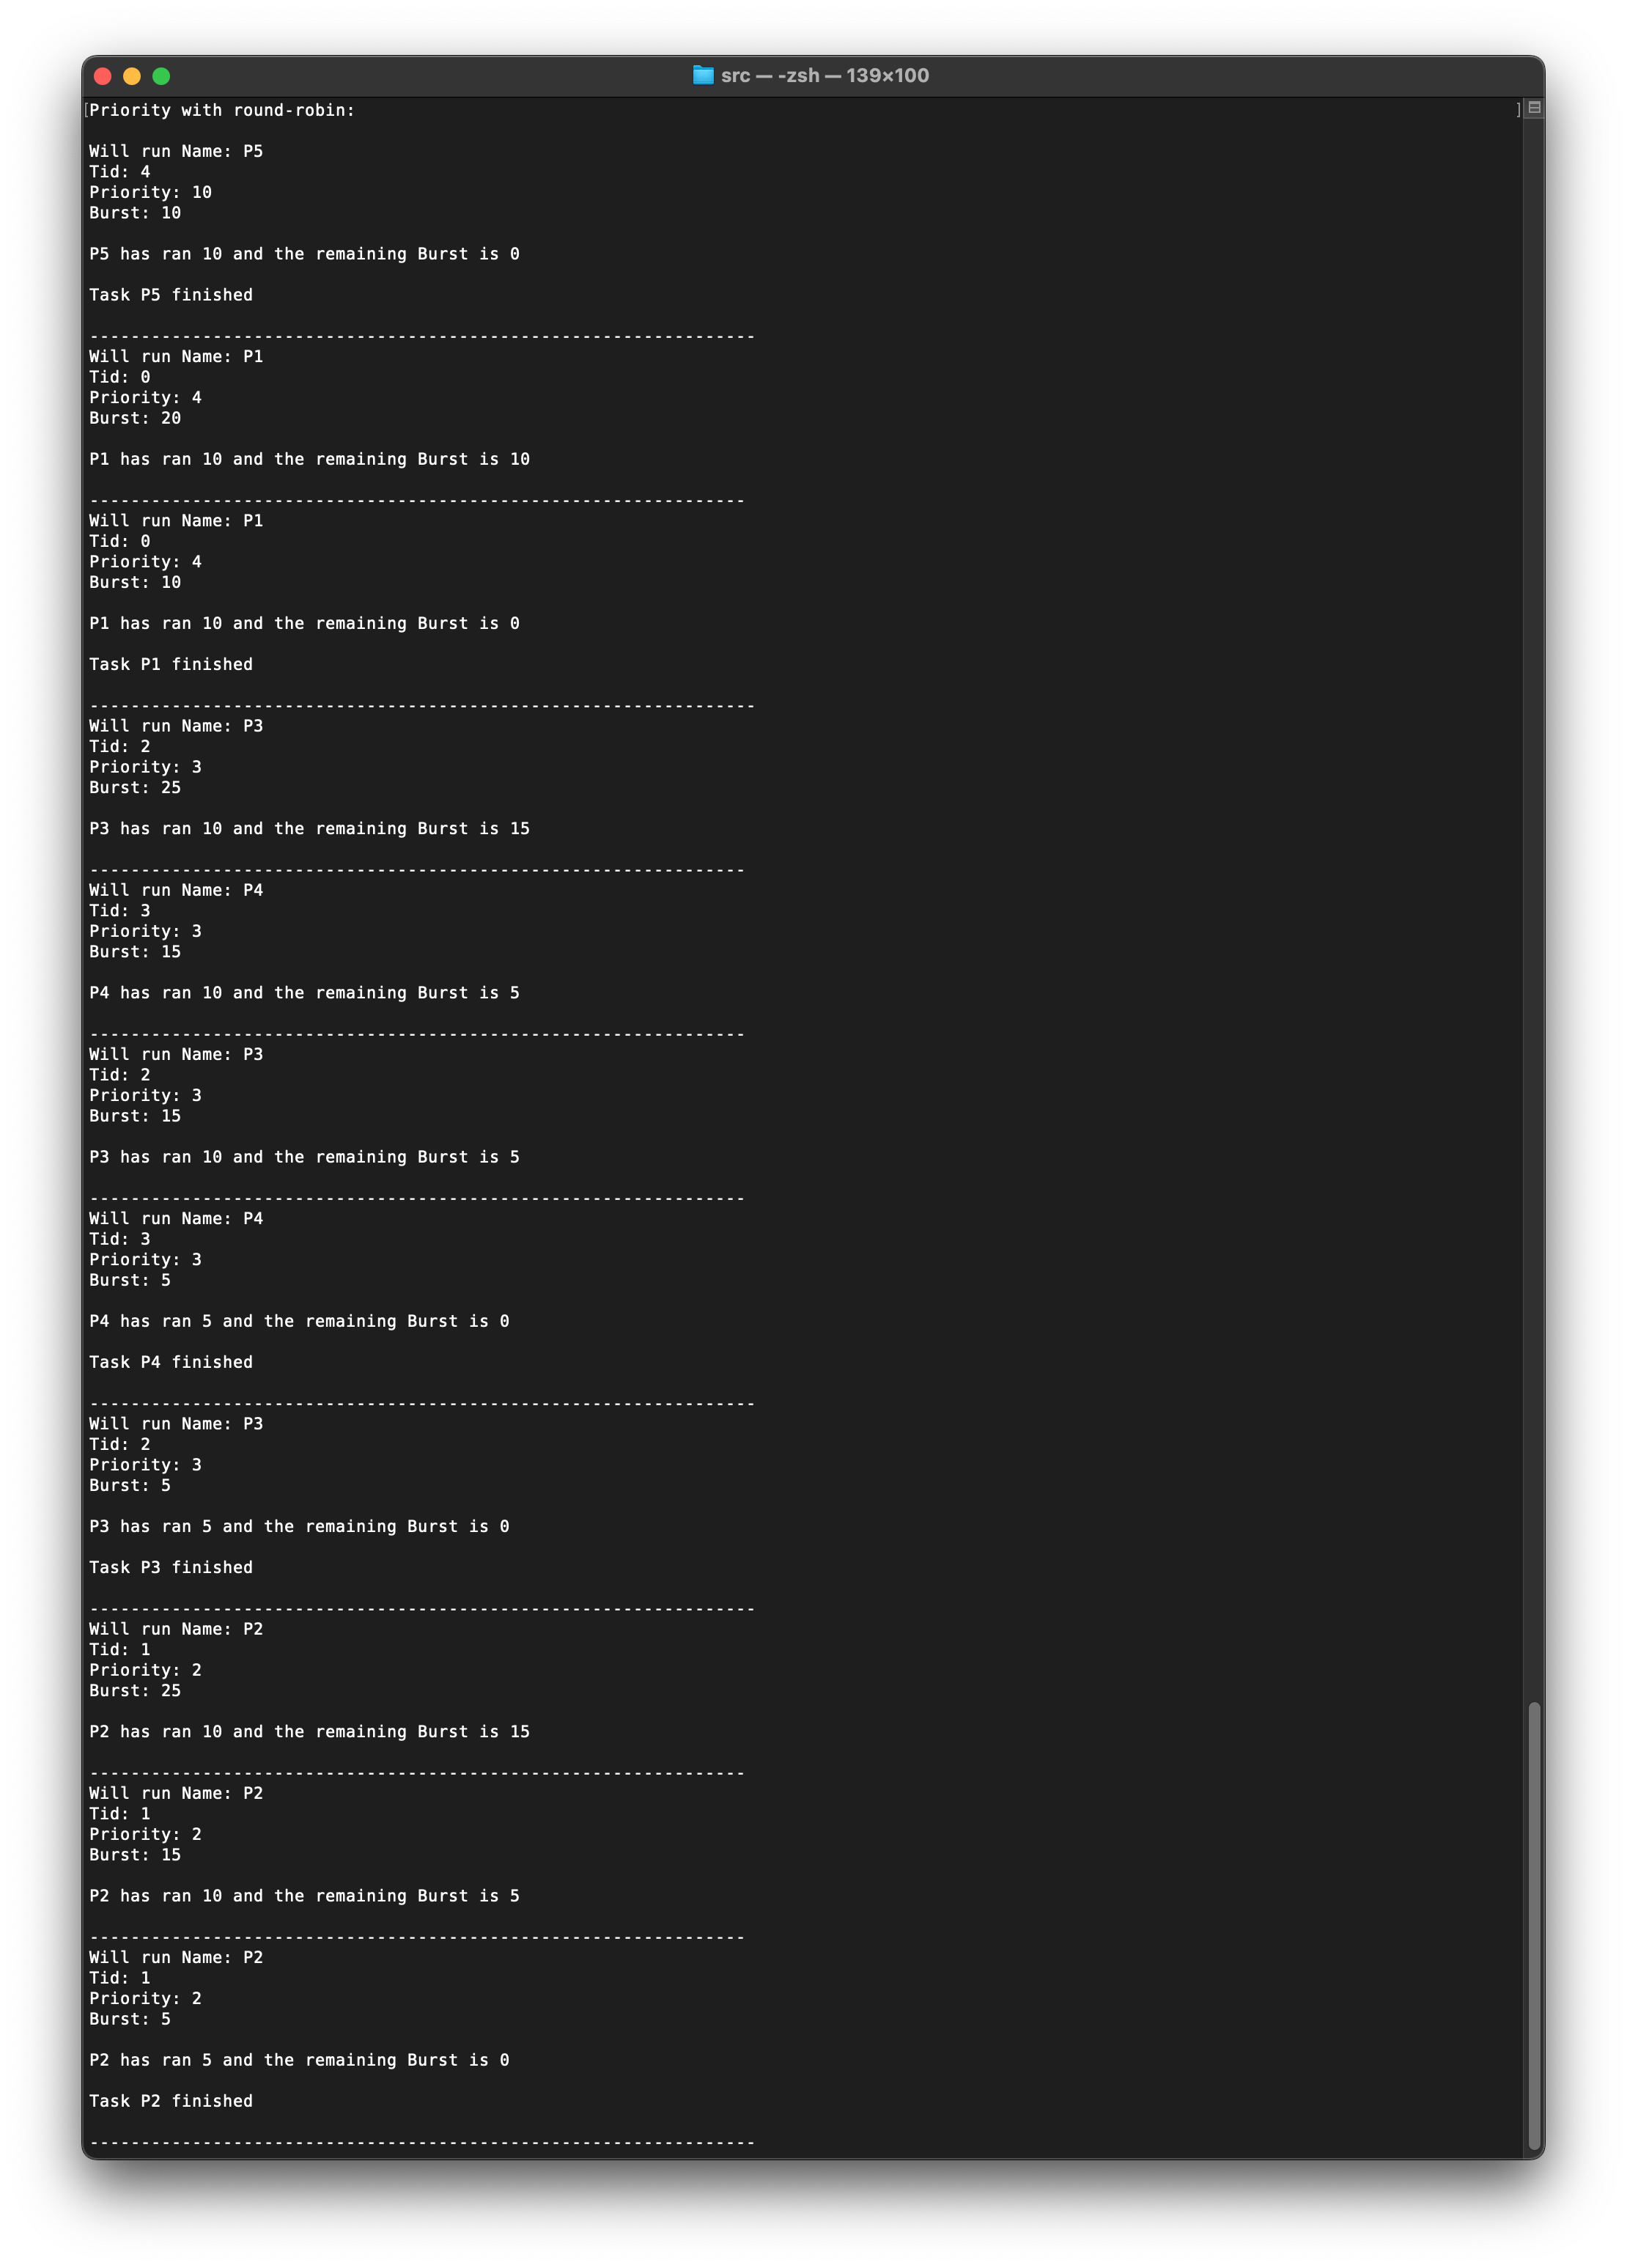
\includegraphics[width=0.9\textwidth]{a5.png}
    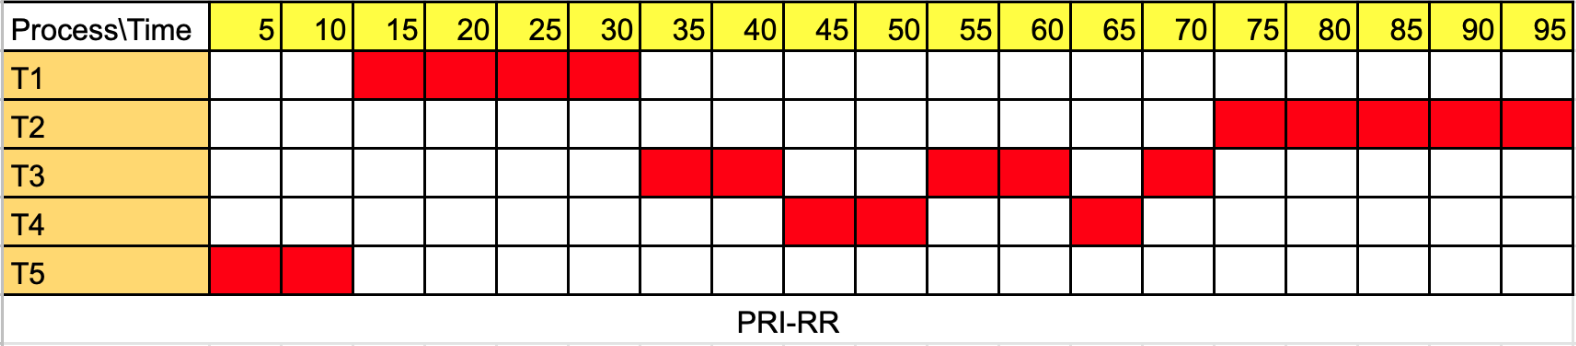
\includegraphics[width=0.9\textwidth]{P5.png}
    
    \end{enumerate}
    More code detail can see in the source code of the project.
    \end{sol}
    \newpage
    \item (\colorbox{yellow}{must be answered by CS 7343 students only}) Consider a variation of round robin scheduling, say NRR scheduling. In NRR scheduling, each process can have its own time quantum, q. The value of q starts out at 40 ms and decreases by 10 ms each time it goes through the round robin queue, until it reaches a minimum of 10 ms. Thus, long jobs get decreasingly shorter time slices.
Analyze this scheduling algorithm for three jobs A, B, and C that arrive in the system having estimated burst times of 100 ms, 120 ms, and 60 ms respectively. Also identify some advantages and disadvantages that are associated with this algorithm.
\begin{sol}
    \hspace*{\fill} \\
    Result:
    \begin{center}
        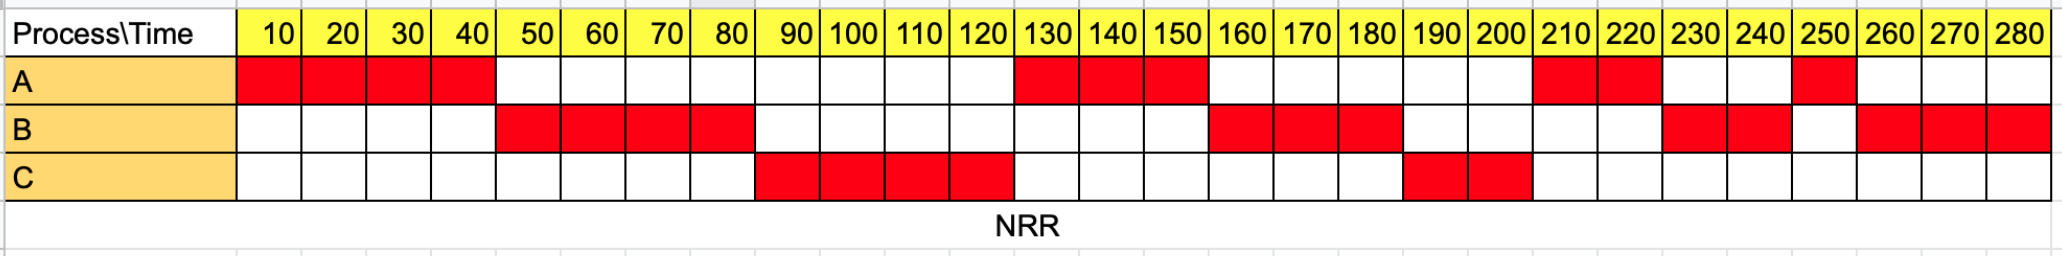
\includegraphics[width=0.9\textwidth]{C.png}
    \end{center}
    In the first round, each of job gets 40 ms.\\
    In the second round, each of job gets 30 ms, however, the job C just need 20ms and job C finished.\\
    In the third round, each of job gets 20 ms, C has ready done. \\
    In the fourth round, job A, job B gets 10 ms, however, A finished.\\
    In the five round, there is only job B left, get 10 ms.\\
    In the six round, job B get 10 ms and finished.\\
    \textbf{Advantages:} At the begin, job will get more quantum, if the burst time of job will not long, it can finish at beginning. Good for the short burst time job. And it can also good for the long burst time job at the beginning.
    \\
    \textbf{Disadvantages:} When quantum is reducing, the job with long burst time will takes too many rounds than normal Round Robin. And the quantum decrease will increasing the switching time.
    
\end{sol}

\end{enumerate}

\end{document}
